\documentclass[a4paper,11pt]{article}

\usepackage{fancyhdr}
\usepackage[dvips]{graphicx}  % for eps and MatLab Diagrams
\usepackage{amsmath}
\usepackage{psfrag,color}
\usepackage[framed]{/Applications/TeX/mcode}

\pagestyle{fancy}

\newcommand{\G}{\mcode{GRIDFIT}}

\begin{document} % Begin Document

% Title
\title{\textsc{Understanding Gridfit}}

% Authors and Contact Information
\author{\textbf{John R. D'Errico}\\
Email: woodchips@rochester.rr.com}

\maketitle

\section{Introduction}

\G{} is a surface modeling tool, fitting a surface of the form
$z(x,y)$ to scattered (or regular) data. As it is not an
interpolant, it allows the existence of replicates in your data with
no problems. What do I mean by an "interpolant"? An interpolant is a
code that is designed to always exactly predict all supplied data.
\mcode{GRIDDATA} and \mcode{INTERP1} are examples of interpolants.
\G{} is more accurately described as an approximant. It produces a
surface which represents the behavior of the supplied data as
closely as possible, allowing for noise in the data and for
replicate data.

A nice feature of \G{} is its ability to smoothly extrapolate beyond
the convex hull of your data, something that \mcode{GRIDDATA} cannot
do.\footnote{except by the slow, memory intensive 'v4' method}
Finally, \G{} does its extrapolation in a well behaved manner,
unlike how polynomial models (for example) might behave in
extrapolation.

\G{} also allows you to build a gridded surface directly from your
data, rather than interpolating a linear approximation to a surface
from a delaunay triangulation.

This document describes the ideas behind \G.

\section{The mechanical and philosophical underpinnings of GRIDFIT}

How does \G{} work? Imagine a thin, flexible plate, attached to your
data points by elastic bands. Each of these elastic bands draws the
plate towards its corresponding data point, stretching only in the 
direction. If your data points were to fall on a simple planar
surface,
\begin{equation}
    z(x,y) = a_0 + a_1 x + a_2 y
 \end{equation}
then the result will be a least squares plane. This works because
the potential energy stored in a elastic band\footnote{perfect,
linearly elastic} will be proportional to the square of its
extension.

Now imagine that the data points do not fall on a plane, but arise
from some curved surface $z(x,y)$. While the plate itself is
flexible, I've allowed it some finite and non-zero bending rigidity
that the user can control. The bands connecting the plate to our
data points will pull the plate into a curved shape, while the
bending rigidity of the plate resists deformation. The relative
stiffness of the plate, as compared to the strength of the elastic
bands will cause some tradeoff between fitting the data as well as
possible and a smooth overall surface. It is this plate stiffness
that allows \G{} to smoothly extrapolate beyond the data itself. Of
course, extrapolation beyond the data will be well behaved, since
the plate will tend to become locally planar wherever there is no
data to deform it.

The tradeoff between stiffness of the plate and the effective spring
constant of the bands connecting the plate to the data allows the
user to choose anything between the extremes of a purely planar fit,
to a crinkly thing that can follow the bumps and hollows of noisy
data.


\section{The methodology of GRIDFIT}

First, lets look at how \G{} predicts a value at any location. Since
the \G{} surface is defined by values at a set of nodes forming a
rectangular lattice, any data point must lie in one of these
rectangular cells of the lattice. (One requirement of \G{} is that
the boundaries of its lattice must form a bounding box for all of
the data supplied in the $(x,y)$ plane.)

Given a point inside a single rectangular cell of the lattice, there
are three methods supplied in \G{} to impute a value at that point.
They are:
\begin{itemize}
  \item Nearest neighbor interpolation
  \item Triangle (linear) interpolation
  \item Bilinear (tensor product linear) interpolation
\end{itemize}

These methods were chosen to be simple to generate, as well as
because they are very "local" methods.  They require no more than a
few local values from the grid to predict the value at each point.
This local nature makes the sparse linear least squares problem as
efficient as possible, by keeping it maximally sparse.

If we think of the surface that will result from \G{} as essentially
a low order spline, it is easy to visualize the idea that
interpolation at any point inside the grid is just a linear
combination of the values at the grid nodes in the locality of the
given point. Thus, we can write the interpolation problem in general
as a linear algebra problem
\begin{equation}
    A\mathbf{x}=\mathbf{y}
\end{equation}
where the vector $\mathbf{x}$ is of length $nx\cdot{}ny$ ($nx$ is
the number of nodes in the $\mathbf{x}$ direction, and $ny$ is the
number of grid nodes in the $\mathbf{y}$ direction.) Thus $A$ has
$n$ rows, corresponding to each data point supplied by the user, and
$nx\cdot{}ny$ columns.

It will not be atypical to expect that there will be more columns
than rows in this "regression" problem. For example, a user with 100
data points might choose to build a gridded surface which has
$100\times100$ nodes. The resulting regression problem will be
massively underdetermined. As such, standard regression techniques,
involving a solution like \mcode{x = A$\backslash{}$y} or \mcode{x =
pinv(A)*y}, will be inappropriate.

The approach that \G{} takes, with its plate-like metaphor, is to
solve a regularized problem. At every node of the surface,
\G{}\footnote{using its default regularization method of 'gradient'}
attempts to force the (first) partial derivatives of the surface in
neighboring cells to be equal. In effect, this results in a second
set of linear equations of the form
\begin{equation}
    B\mathbf{x} = \mathbf{0}
\end{equation}
where the derivatives are approximated using finite differences of
the surface at neighboring nodes.

The main alternative regularization method in \G{} is the
'laplacian' method. It attempts to force the sum of second partial
derivatives to zero. This is actually closely related to the
gradient method, but with a subtly significant difference. Either
method will work nicely. (The 'springs' regularizer for \G{} is a
flawed one, at least in my humble opinion. I'd generally recommend
not using it without care. I've left it in the code because it has
interesting properties in extrapolation.)

The result of any of these regularizers is a system of the form
$B\mathbf{x}=\mathbf{0}$. Coupled with the interpolation system,
$A\mathbf{x}=\mathbf{y}$, we solve them in combination using a
simple trick. First, I scale $A$ and $B$ so that each matrix has a
unit 1-norm. This helps to eliminate scaling problems with the
derivatives. Then I solve for the vector $\mathbf{x}$ such that
\begin{equation}
    \|(A\mathbf{x}-\mathbf{y})\|^2 + \lambda\|B\mathbf{x}\|^2
\end{equation}
is minimized. Note that the parameter $\lambda$, nominally 1 as a
default in \G, allows the user to control the relative plate
"stiffness". As $\lambda$ approaches zero, the plate becomes as
flexible as possible. Stiffer plates are modeled by larger values,
$\lambda>1$.



\section{Tricks with tiles}

What can you do when a \G{} problem is simply too large even for the
sparse matrix abilities of MATLAB? This is where the tiling
abilities of \G{} become valuable. What do I mean by tiling? An
example might be appropriate.

\begin{lstlisting}
    >> nodes = linspace(0,1,100);
    >> tic,...
    zg=gridfit(rand(100,1),rand(100,1),rand(100,1),nodes,nodes);...
    toc
    Elapsed time is 5.814102 seconds.
    >>
    >> nodes = linspace(0,1,200);
    >> tic,...
    zg=gridfit(rand(100,1),rand(100,1),rand(100,1),nodes,nodes);...
    toc
    Elapsed time is 27.118945 seconds.
\end{lstlisting}
\bigskip

To solve for a $100\times100$ grid, \G{} must solve for 10000
unknown parameters using sparse linear algebra. A $200\times200$
grid is nominally 4 times as large, and it took my computer a bit
more than $4\times$ as long to solve. However, a $2000\times2000$
grid will probably take much more than 400 times as long to solve as
a $100\times100$ grid. It will likely take very much longer, if it
runs at all without exceeding the memory limits, due to the much
slower access times for virtual memory. For example, my computer
took 1020 seconds to solve a $500\times500$ problem.
\begin{lstlisting}
    >> nodes = linspace(0,1,500);
    >> tic,...
    zg=gridfit(rand(100,1),rand(100,1),rand(100,1),nodes,nodes);...
    toc
    Elapsed time is 1020.657834 seconds.
\end{lstlisting}
\bigskip

A trick that can work, IF you have enough data to adequately
populate each tile, is to break down the domain of a large grid into
smaller chunks, each of which can be quickly populated by \G. Then
\G{} composes each chunk into the whole surface. To smooth out any
artifacts at the edges of each tile, \G{} allows the tiles some
fractional overlap, interpolating between them in the overlapped
region. Thus the tiled solution below was accomplished with
essentially no dips into virtual memory, so it took far less time to
generate.

\begin{lstlisting}
    >> nodes = linspace(0,1,500);
    >> tic,...
    zg=gridfit(rand(100,1),rand(100,1),rand(100,1),nodes,nodes,...
    'tilesize',200,'overlap',0.2);...
    toc
    Elapsed time is 211.946853 seconds.
\end{lstlisting}
\bigskip

Note: these random surfaces were generated purely to show speed of
estimation. They are of course purely garbage. Also, only 100 data
points may well be inadequate to estimate a tiled surface. \G{} is
not strongly dependent on the number of data points for its speed,
so that number did not have an impact on the speed of estimation.

A picture:

\begin{lstlisting}
    % Users of gridfit who have really huge problems now have
    % an option. I'll generate a large amount of data,
    % and hope to model a fairly large grid - 800 x 800. This
    % would normally require gridfit to solve a system of
    % equations with 640,000 unknowns. It would probably be too
    % large of a problem for my computer, were I to use gridfit
    % on the full problem. Gridfit allows you to break the problem
    % into smaller tiles if you choose. In this case each tile
    % is 120x120, with a 25% (30 element) overlap between tiles.

    % Relax, this demo may take a couple of minutes to run!!!!

    n = 100000;
    x = rand(n,1);
    y = rand(n,1);
    z = x+y+sin((x.^2+y.^2)*10);

    xnodes = 0:.00125:1;
    ynodes = xnodes;

    [zg,xg,yg] = gridfit(x,y,z,xnodes,ynodes,'tilesize',...
    120,'overlap',0.25);

    surf(xg,yg,zg)
    shading interp
    colormap(jet(256))
    camlight right
    lighting phong
    title 'Tiled gridfit'
\end{lstlisting}

\begin{figure}
\centering
    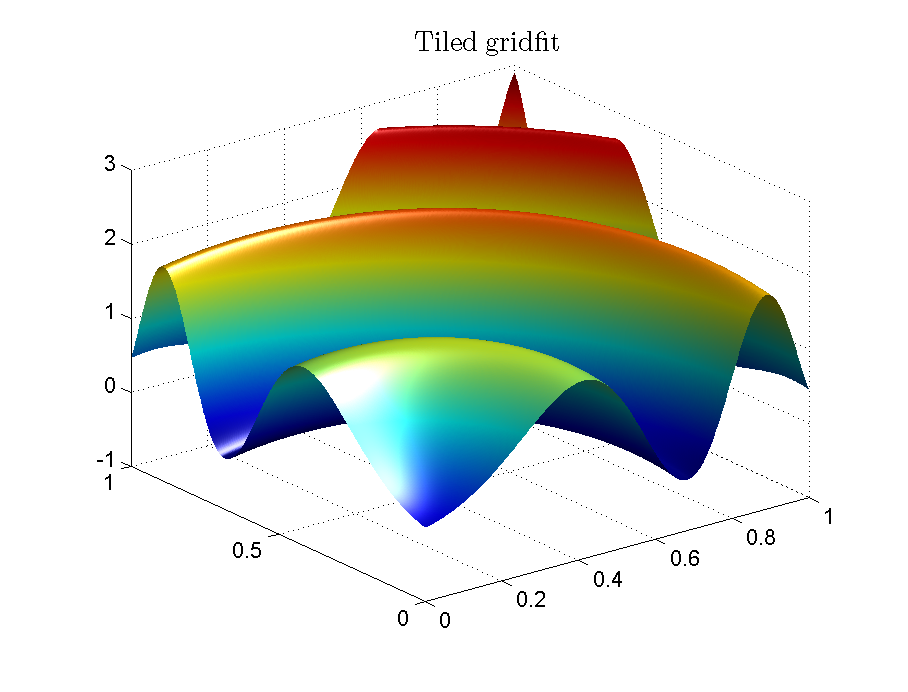
\includegraphics[width=5in]{gfit.eps}
        \caption{An Example}
\end{figure}



\end{document}
